\documentclass[tikz,border=6pt]{standalone}
\usepackage[T1]{fontenc}
\usepackage{newtxtext,newtxmath}
\usepackage{tikz}
\usetikzlibrary{arrows.meta,positioning,calc,backgrounds}

\definecolor{ink}{HTML}{172033}
\definecolor{greyLine}{HTML}{9CA3AF}
\definecolor{greyFill}{HTML}{F3F4F6}
\definecolor{qkC}{HTML}{B91C1C}
\definecolor{ovC}{HTML}{0B7285}
\definecolor{steerC}{HTML}{2E7D32}

\tikzset{
  >={Latex[length=2.4mm,width=1.7mm]},
  ctitle/.style={font=\bfseries,text=ink,align=center},
  note/.style={font=\scriptsize,text=steerC,align=center},
  rowlab/.style={font=\small\bfseries,align=center},
  poslab/.style={font=\scriptsize\bfseries,text=ink,align=center},
  feat/.style={draw,line width=0.8pt,rounded corners=2pt,minimum width=10mm,
    minimum height=8.5mm,font=\small\bfseries,text=ink,inner sep=1pt},
  abl/.style={draw=greyLine,densely dashed,line width=0.8pt,rounded corners=2pt,
    minimum width=10mm,minimum height=8.5mm,font=\small\bfseries,text=greyLine,inner sep=1pt,fill=white},
  knob/.style={circle,draw=steerC,fill=steerC,text=white,font=\tiny\bfseries,
    inner sep=0.3pt,minimum size=4mm,line width=0.4pt},
  keytxt/.style={font=\scriptsize,text=ink,align=left,anchor=west},
}

\begin{document}
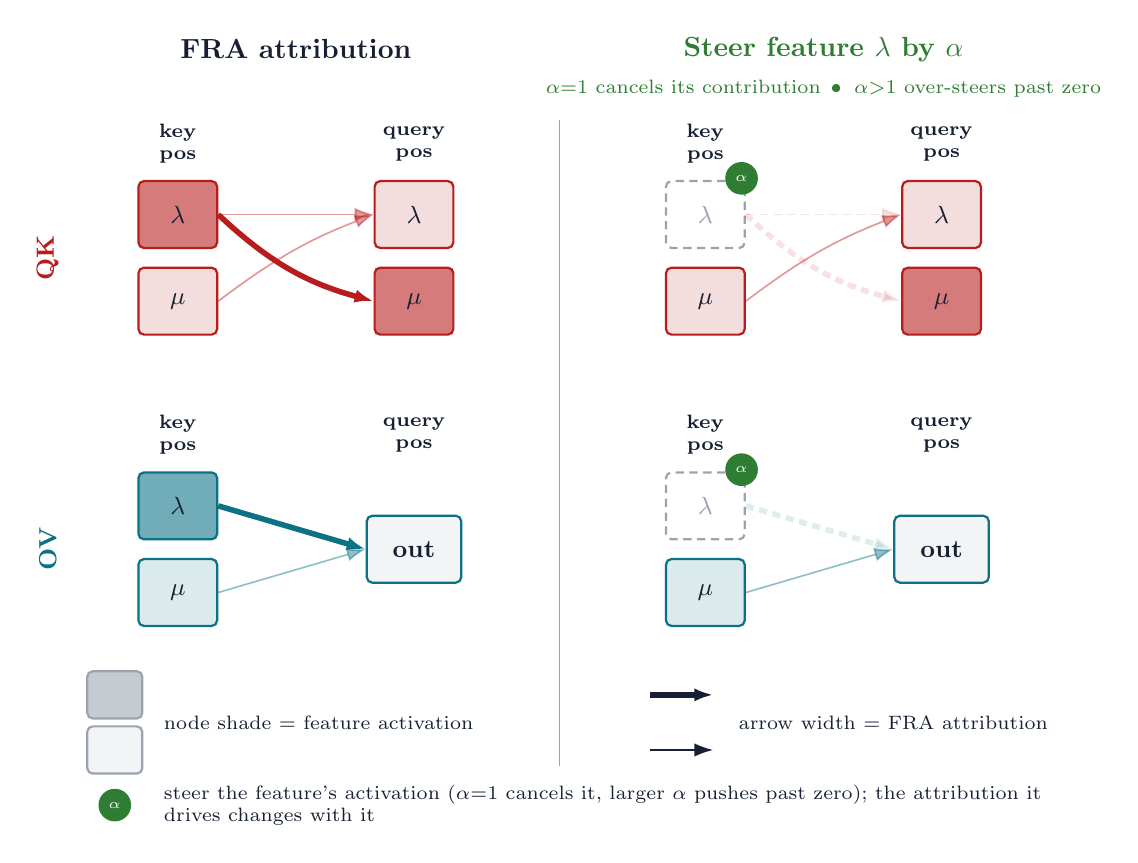
\begin{tikzpicture}[x=1mm,y=1mm]

% ---------- titles ----------
\node[ctitle] at (33,95) {FRA attribution};
\node[ctitle,text=steerC] at (100,95) {Steer feature $\lambda$ by $\alpha$};
\node[note] at (100,90) {$\alpha{=}1$ cancels its contribution \,\textbullet\, $\alpha{>}1$ over-steers past zero};
\draw[greyLine,line width=0.4pt] (66.5,4) -- (66.5,86);

% ---------- shared row labels ----------
\node[rowlab,text=qkC,rotate=90] at (1.5,68.5) {QK};
\node[rowlab,text=ovC,rotate=90] at (1.5,31.5) {OV};

% ================= LEFT COLUMN (attribution) =================
\node[poslab] at (18,83) {key\\pos}; \node[poslab] at (48,83) {query\\pos};
\node[feat,draw=qkC,fill=qkC!58] (Lk1) at (18,74) {$\lambda$};
\node[feat,draw=qkC,fill=qkC!15] (Lk2) at (18,63) {$\mu$};
\node[feat,draw=qkC,fill=qkC!15] (Lq1) at (48,74) {$\lambda$};
\node[feat,draw=qkC,fill=qkC!58] (Lq2) at (48,63) {$\mu$};
\draw[->,qkC,line width=0.6pt,opacity=0.45] (Lk1.east) -- (Lq1.west);
\draw[->,qkC,line width=0.6pt,opacity=0.45] (Lk2.east) to[bend left=8] (Lq1.west);
\draw[->,qkC,line width=2.0pt] (Lk1.east) to[bend right=14] (Lq2.west);
\node[poslab] at (18,46) {key\\pos}; \node[poslab] at (48,46) {query\\pos};
\node[feat,draw=ovC,fill=ovC!58] (Lo1) at (18,37) {$\lambda$};
\node[feat,draw=ovC,fill=ovC!15] (Lo2) at (18,26) {$\mu$};
\node[feat,draw=ovC,fill=greyFill,minimum width=12mm] (Lout) at (48,31.5) {out};
\draw[->,ovC,line width=2.0pt] (Lo1.east) -- (Lout.west);
\draw[->,ovC,line width=0.6pt,opacity=0.45] (Lo2.east) -- (Lout.west);

% ================= RIGHT COLUMN (steer lambda) =================
\node[poslab] at (85,83) {key\\pos}; \node[poslab] at (115,83) {query\\pos};
\node[abl] (Rk1) at (85,74) {$\lambda$};
\node[knob] at ([xshift=4.6mm,yshift=4.6mm]Rk1.center) {$\alpha$};
\node[feat,draw=qkC,fill=qkC!15] (Rk2) at (85,63) {$\mu$};
\node[feat,draw=qkC,fill=qkC!15] (Rq1) at (115,74) {$\lambda$};
\node[feat,draw=qkC,fill=qkC!58] (Rq2) at (115,63) {$\mu$};
\draw[->,qkC,line width=0.6pt,densely dashed,opacity=0.13] (Rk1.east) -- (Rq1.west);
\draw[->,qkC,line width=0.6pt,opacity=0.45] (Rk2.east) to[bend left=8] (Rq1.west);
\draw[->,qkC,line width=2.0pt,densely dashed,opacity=0.13] (Rk1.east) to[bend right=14] (Rq2.west);
\node[poslab] at (85,46) {key\\pos}; \node[poslab] at (115,46) {query\\pos};
\node[abl] (Ro1) at (85,37) {$\lambda$};
\node[knob] at ([xshift=4.6mm,yshift=4.6mm]Ro1.center) {$\alpha$};
\node[feat,draw=ovC,fill=ovC!15] (Ro2) at (85,26) {$\mu$};
\node[feat,draw=ovC,fill=greyFill,minimum width=12mm] (Rout) at (115,31.5) {out};
\draw[->,ovC,line width=2.0pt,densely dashed,opacity=0.13] (Ro1.east) -- (Rout.west);
\draw[->,ovC,line width=0.6pt,opacity=0.45] (Ro2.east) -- (Rout.west);

% ================= LEGEND =================
\node[feat,draw=greyLine,fill=greyLine!58,minimum width=7mm,minimum height=6mm] at (10,13) {};
\node[feat,draw=greyLine,fill=greyLine!13,minimum width=7mm,minimum height=6mm] at (10,6) {};
\node[keytxt] at (15,9.5) {node shade $=$ feature activation};
\draw[->,ink,line width=2.0pt] (78,13) -- (86,13);
\draw[->,ink,line width=0.6pt] (78,6) -- (86,6);
\node[keytxt] at (88,9.5) {arrow width $=$ FRA attribution};
\node[knob] at (10,-1) {$\alpha$};
\node[keytxt,text width=112mm] at (15,-1) {steer the feature's activation ($\alpha{=}1$ cancels it, larger $\alpha$ pushes past zero); the attribution it drives changes with it};

\end{tikzpicture}
\end{document}
